\begin{tikzpicture}[scale=1,x=1em,y=1em]
\node at (0,0) {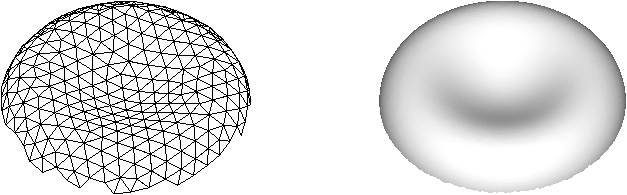
\includegraphics[width=11em]{./figures/network2continuum.pdf}};
\draw[very thick, <->, >=stealth'] (-2,0.5) node[text width=4.5em,left] {\tiny 弹簧常数, 弯曲常数\vspace{-1em} 体积约束, 面积约束} -- (2, 0.5) node[text width=4.5em, right] {\tiny 剪切模量, 压缩模量\vspace{-1em} 杨氏模量, 弯曲刚度};
%\draw[very thick, <->, >=stealth'] (-0.8,0) -- (0.8, 0);
\draw[very thick, <->, >=stealth'] (-2,-4.5) node[left]{\scriptsize 粒子模型} -- (2, -4.5) node[right] {\scriptsize 连续模型};;
\end{tikzpicture}
